%% Copernicus Publications Manuscript Preparation Template for LaTeX Submissions
%% ---------------------------------
%% This template should be used for copernicus.cls
%% The class file and some style files are bundled in the Copernicus Latex Package, which can be downloaded from the different journal webpages.
%% For further assistance please contact Copernicus Publications at: production@copernicus.org
%% https://publications.copernicus.org/for_authors/manuscript_preparation.html


%% Please use the following documentclass and journal abbreviations for discussion papers and final revised papers.

%% 2-column papers and discussion papers
\documentclass[tc, manuscript]{copernicus}



%% Journal abbreviations (please use the same for discussion papers and final revised papers)


% Advances in Geosciences (adgeo)
% Advances in Radio Science (ars)
% Advances in Science and Research (asr)
% Advances in Statistical Climatology, Meteorology and Oceanography (ascmo)
% Annales Geophysicae (angeo)
% Archives Animal Breeding (aab)
% ASTRA Proceedings (ap)
% Atmospheric Chemistry and Physics (acp)
% Atmospheric Measurement Techniques (amt)
% Biogeosciences (bg)
% Climate of the Past (cp)
% DEUQUA Special Publications (deuquasp)
% Drinking Water Engineering and Science (dwes)
% Earth Surface Dynamics (esurf)
% Earth System Dynamics (esd)
% Earth System Science Data (essd)
% E&G Quaternary Science Journal (egqsj)
% European Journal of Mineralogy (ejm)
% Fossil Record (fr)
% Geochronology (gchron)
% Geographica Helvetica (gh)
% Geoscience Communication (gc)
% Geoscientific Instrumentation, Methods and Data Systems (gi)
% Geoscientific Model Development (gmd)
% History of Geo- and Space Sciences (hgss)
% Hydrology and Earth System Sciences (hess)
% Journal of Micropalaeontology (jm)
% Journal of Sensors and Sensor Systems (jsss)
% Magnetic Resonance (mr)
% Mechanical Sciences (ms)
% Natural Hazards and Earth System Sciences (nhess)
% Nonlinear Processes in Geophysics (npg)
% Ocean Science (os)
% Primate Biology (pb)
% Proceedings of the International Association of Hydrological Sciences (piahs)
% Scientific Drilling (sd)
% SOIL (soil)
% Solid Earth (se)
% The Cryosphere (tc)
% Weather and Climate Dynamics (wcd)
% Web Ecology (we)
% Wind Energy Science (wes)


%% \usepackage commands included in the copernicus.cls:
%\usepackage[german, english]{babel}
%\usepackage{tabularx}
%\usepackage{cancel}
%\usepackage{multirow}
%\usepackage{supertabular}
%\usepackage{algorithmic}
%\usepackage{algorithm}
%\usepackage{amsthm}
%\usepackage{float}
\usepackage{subfig}
%\usepackage{rotating}


\begin{document}

\title{DeepBedMap: Using a deep neural network to better resolve the bed topography of Antarctica}


% \Author[affil]{given_name}{surname}

\Author[1]{Wei Ji}{Leong}
\Author[1]{Huw Joseph}{Horgan}

\affil[1]{Antarctic Research Centre, Victoria University of Wellington, Wellington, New Zealand}

%% The [] brackets identify the author with the corresponding affiliation. 1, 2, 3, etc. should be inserted.

%% If an author is deceased, please mark the respective author name(s) with a dagger, e.g. "\Author[2,$\dag$]{Anton}{Aman}", and add a further "\affil[$\dag$]{deceased, 1 July 2019}".

%% If authors contributed equally, please mark the respective author names with an asterisk, e.g. "\Author[2,*]{Anton}{Aman}" and "\Author[3,*]{Bradley}{Bman}" and add a further affiliation: "\affil[*]{These authors contributed equally to this work.}".


\correspondence{W. J. Leong (weiji.leong@vuw.ac.nz)}

\runningtitle{DeepBedMap Antarctica}

\runningauthor{W. J. Leong and H. J. Horgan}





\received{}
\pubdiscuss{} %% only important for two-stage journals
\revised{}
\accepted{}
\published{}

%% These dates will be inserted by Copernicus Publications during the typesetting process.


\firstpage{1}

\maketitle



\begin{abstract}
To better resolve the bed elevation of Antarctica, we present DeepBedMap - a novel machine learning method that produces realistic Antarctic bed topography from multiple remote sensing data inputs.
Our super-resolution deep convolutional neural network model is trained on scattered regions in Antarctica where high resolution (250 m) groundtruth bed elevation grids are available.
The model is then used to generate high resolution bed topography in less well surveyed areas.
DeepBedMap improves on previous interpolation methods by not restricting itself to a low spatial resolution (1000 m) BEDMAP2 raster image as its prior.
It takes in additional high spatial resolution datasets, such as ice surface elevation, velocity and snow accumulation to better inform the bed topography even in the absence of ice-thickness data from direct ice-penetrating radar surveys.
Our DeepBedMap model is based on an adapted Enhanced Super Resolution Generative Adversarial Network architecture, chosen to minimize per-pixel elevation errors while producing realistic topography.
The final product is a four times upsampled (250 m) bed elevation model of Antarctica that can be used by glaciologists interested in the subglacial terrain, and by ice sheet modellers wanting to run catchment or continent-scale ice sheet model simulations.
We show that DeepBedMap offers a more realistic topographic roughness profile compared to a standard bicubic interpolated BEDMAP2 and BedMachine Antarctica, and envision it to be used where a high resolution bed elevation model is required.
\end{abstract}


\copyrightstatement{This work is distributed under the Creative Commons Attribution 4.0 License}


\introduction  %% \introduction[modified heading if necessary]

The bed of the Antarctic ice sheets is one of the most challenging surfaces on Earth to map due to the thick layer of ice cover.
Knowledge of bed elevation is however essential for estimating the volume of ice currently stored in the ice sheets, and for input to the numerical models that are used to estimate the contribution ice sheets are to likely to make to sea level in the coming century.
The Antarctic ice sheet is estimated to hold a sea level equivalent (SLE) of 57.9 ± 0.9 m \citep{MorlighemDeepglacialtroughs2019}.
Between 2012 and 2017, the Antarctic Ice Sheet was losing mass at an average rate of 219 ± 43 Gt yr$^{-1}$ (0.61 ± 0.12 mm yr$^{-1}$ SLE), with most of the ice loss attributed to the acceleration, retreat and rapid thinning of major West Antarctic Ice Sheet outlet glaciers \citep{TheIMBIEteamMassbalanceAntarctic2018}.
Bed elevation exerts additional controls on ice flow by routing subglacial water, and providing frictional resistance to flow \citep{SiegertMacroscalebedroughness2004}.
Bed roughness, especially at short-wavelengths, exerts a frictional force against the flow of ice, making it an important influence on ice velocity \citep{BinghamDiverselandscapesPine2017,FalciniQuantifyingbedroughness2018}.
The importance of bed elevation has led to major efforts to compile bed elevation models of Antarctica, notably with the BEDMAP1 \citep{LytheBEDMAPnewice2001} and BEDMAP2 \citep{FretwellBedmap2improvedice2013} products.
A need for higher spatial resolution Digital Elevation Model (DEM) is also apparent, as ice sheet models move to using sub-kilometer grids in order to quantify glacier ice flow dynamics more accurately \citep{Grahamhighresolutionsyntheticbed2017}.
Finer grids are especially important at the ice sheet's grounding zone where adaptive mesh refinement schemes have focused on \citep[e.g.][]{CornfordAdaptivemeshrefinement2016}, and attention to the bed roughness component is imperative for proper modelling of fast flowing outlet glaciers \citep{DurandImpactbedrockdescription2011,NiasContrastingmodelledsensitivity2016}.
Here we address the challenge of producing a high resolution DEM while preserving a realistic representation of the bed terrain's roughness.

Estimating bed elevation directly from geophysical observations primarily uses ice penetrating radar methods \citep[e.g.][]{RobinRadioechoexploration1970}.
Airborne radar methods enable reliable along track estimates with low uncertainty (around the 1\% level) introduced by imperfect knowledge of the firn and ice velocity structure, with some potential uncertainty introduced by picking the bed return.
Radar derived bed estimates remain limited in their geographic coverage \citep{FretwellBedmap2improvedice2013}, and are typically anisotropic in their coverage, with higher spatial sampling in the along track direction than between tracks.

To overcome these limitations, indirect methods of estimating bed elevation have been developed, which use surface observations combined with glaciological process knowledge to determine ice thickness \citep[e.g.][]{vanPeltiterativeinversemethod2013}.
A non-linear relationship exists between the thickness of glaciers, ice streams and ice sheets and how they flow \citep{Raymondrelationshipsurfacebasal2005}, meaning one can theoretically use a well resolved surface to infer bed properties \citep[e.g.][]{Farinottimethodestimateice2009}.
Using surface observation inputs, such as the glacier outline, surface digital elevation models, surface mass balance, surface rate of elevation change, and surface ice flow velocity, various models have been tested in the Ice Thickness Models Intercomparison eXperiment \citep[ITMIX,][]{FarinottiHowaccurateare2017} to determine ice thickness (surface elevation minus bed elevation).
While significant inter-model uncertainties do exist, they can be mitigated by combining several models in an ensemble to provide a better consensus estimate \citep{Farinotticonsensusestimateice2019}.
On a larger scale, the inverse technique has also been applied to the Greenland \citep{MorlighemBedMachinev3Complete2017} and Antarctic \citep{MorlighemDeepglacialtroughs2019} ice sheets, specifically using the mass conservation approach \citep{Morlighemmassconservationapproach2011}.

We present a deep neural network method that belongs to the inverse modelling category and is trained on direct ice-penetrating radar observations over Antarctica.
An artificial neural network, loosely based on biological neural networks, is a system made up of neurons.
Each neuron comprises of a simple mathematical function that takes an input to produce an output value, and neural networks work by combining many of these neurons together.
The term deep neural network is used when there is not a direct function mapping between the input data and final output, but two or more layers that are connected to one another \citep[see][for a review]{LeCunDeeplearning2015}.
They are trained using backpropagation, a procedure whereby the weights or parameters of the neurons' connections are adjusted, so as to minimize the error between the groundtruth and output of the neural network \citep{RumelhartLearningrepresentationsbackpropagating1986}. Similar work has been done before using artificial neural networks for estimating bed topography \citep[e.g.][]{ClarkeNeuralNetworksApplied2009,MonnierInferencebedtopography2018}, but to our knowledge, none so far in the glaciological community have attempted to use convolutional neural networks that works in a more spatially-aware, 2-dimensional setting.
Convolutional neural networks differ from standard artificial neural networks in that they use kernels or filters in place of regular neurons \citep[again, see][for a review]{LeCunDeeplearning2015}.
The techniques we employ are prevalent in the computer vision community, having existed since the 1980s \citep{FukushimaNeocognitronnewalgorithm1982,LeCunBackpropagationAppliedHandwritten1989} and are commonly used in visual pattern recognition tasks \citep[e.g.][]{LecunGradientbasedlearningapplied1998,KrizhevskyImageNetClassificationDeep2012}.
Our main contributions are twofold:
1) Present a high resolution (250 m) bed elevation map of Antarctica that goes beyond the 1 km resolution of BEDMAP2 \citep{FretwellBedmap2improvedice2013};
2) Design a deep convolutional neural network to integrate as many remote sensing datasets as possible which are relevant for estimating Antarctica's bed topography.
We name the neural network "DeepBedMap", and the resulting digital elevation model (DEM) product as "DeepBedMap\_DEM".


\section{Related Work}

\subsection{Super-Resolution} \label{section:superresolution}

Super-Resolution involves the processing of a low resolution raster image into a higher resolution one \citep{TsaiMultiframeimagerestoration1984}.
The idea is similar to the work on enhancing regular photographs to look crisper.
The problem is especially ill-posed because a specific low resolution input can correspond to many possible high resolution outputs, resulting in the development of several different algorithms aimed at solving this challenge \citep[see][for a review]{NasrollahiSuperresolutioncomprehensivesurvey2014}.
One promising approach is to use deep neural networks \citep{LeCunDeeplearning2015} to learn an end-to-end mapping between the low and high resolution images, a method coined Super-Resolution Convolutional Neural Network \citep[SRCNN,][]{DongImageSuperResolutionUsing2014}.
Since the development of SRCNN, multiple advances have been made to improve the perceptual quality of super resolution neural networks \cite[see][for a review]{YangDeepLearningSingle2018}.
One way is to use a better loss function, also known as a cost function.
A loss function is a mathematical function that represents the error between the output of the neural network and the groundtruth (see also Appendix \ref{appendix:A}).
By having an adversarial component in its loss function, the Super-Resolution Generative Adversarial Network \citep[SRGAN,][]{LedigPhotoRealisticSingleImage2016} manages to produce super resolution images with finer perceptual details.
A Generative Adversarial Network \citep{GoodfellowGenerativeAdversarialNetworks2014} consists of two neural networks, a Generator and a Discriminator.
A common analogy used is to treat the Generator as an artist that produces imitation paintings, and the Discriminator as an art critic that determines the authenticity of the paintings.
The artist wants to fool the critic into believing its paintings are real, while the critic tries to identify problems with the painting.
Over time, the artist or generator model learns to improve itself based on the critic's judgement, producing authentic looking paintings with high perceptual quality.
Perceptual quality is the extent to which an image looks like a valid natural image, usually as judged by a human.
In this case, perceptual quality is quantified mathematically by the Discriminator or critic taking into account high level features of an image like contrast, texture, etc.
Another way to improve performance is by reconfiguring the neural network's architecture, wherein the layout or building blocks of the neural network are changed.
By removing unnecessary model components and adding residual connections \citep{HeDeepResidualLearning2015}, the Enhanced Deep Super-Resolution network \citep[EDSR,][]{LimEnhancedDeepResidual2017} features a deeper neural network model that has better performance than older models.
For the DeepBedMap model, we choose to adapt an Enhanced Super-Resolution Generative Adversarial Network \citep[ESRGAN,][]{WangESRGANEnhancedSuperResolution2018} that brings together the ideas mentioned above.
This approach produces state of the art perceptual quality and won the 2018 Perceptual Image Restoration and Manipulation Challenge on Super-Resolution (Third Region) \citep{Blau2018PIRMChallenge2018}.

\subsection{Network Conditioning} \label{section:networkconditioning}

Network conditioning means having a neural network process one source of information in the context of other sources \citep{DumoulinFeaturewisetransformations2018}.
In a geographic context, conditioning is akin to using not just one layer, but also other relevant layers with meaningful links to provide additional information to the task at hand.
Many ways exist to insert extra conditional information into a neural network, such as concatenation-based conditioning, conditional biasing, conditional scaling, and conditional affine transformations \citep{DumoulinFeaturewisetransformations2018}.
We choose to use the concatenation-based conditioning approach, whereby all of the individual raster images are concatenated together channel-wise, much like the individual bands of a multispectral satellite image.
This was deemed the most appropriate conditioning method as all the contextual remote sensing datasets are raster grid images, and also because this approach aligns with related work in the remote sensing field.

An example similar to this DEM super-resolution problem is the classic problem of pan-sharpening, whereby a blurry low resolution multispectral image conditioned with a high resolution panchromatic image can be turned into a high resolution multispectral image.
There is ongoing research into the use of deep convolutional neural networks for pan-sharpening \citep{MasiPansharpeningConvolutionalNeural2016,ScarpaTargetAdaptiveCNNBasedPansharpening2018}, sometimes with the incorporation of specific domain-knowledge \citep{YangPanNetDeepNetwork2017}, all of which show promising improvements over classical image processing methods.
More recently, generative adversarial networks \citep{GoodfellowGenerativeAdversarialNetworks2014} have been used in the conditional sense for general image-to-image translation tasks \citep[e.g.][]{IsolaImagetoImageTranslationConditional2016,ParkSemanticImageSynthesis2019}, and also for producing more realistic pan-sharpened satellite images \citep{LiuPSGANGenerativeAdversarial2018}.
Our DeepBedMap model builds upon these ideas and other related DEM super-resolution work \citep{XuNonlocalsimilaritybased2015,ChenConvolutionalNeuralNetwork2016}, while incorporating extra conditional information specific to the cryospheric domain for resolving the bed elevation of Antarctica.


\section{Data and Methods}

\subsection{Data Preparation} \label{section:datapreparation}

Our convolutional neural network model works on 2D images, so we have to ensure all the datasets are in a suitable raster grid format.
Groundtruth bed elevation points picked from radar surveys (see Table \ref{table:groundtruthdata}) are first compiled together onto a common Antarctic Stereographic Projection (EPSG:3031) using the WGS84 datum, reprojecting where necessary.
These points are then gridded onto a 250 m spatial resolution (pixel-node registered) grid.
We preprocess the points first using Generic Mapping Tools v6.0 \citep[GMT6,][]{WesselGenericMappingTools2019}, computing the median elevation for each pixel block in a regular grid.
The preprocessed points are then run through an adjustable tension continuous curvature spline function with a tension factor set to 0.35 to produce a digital elevation model grid.
This grid is further post-processed to mask out pixels that are more than 3 pixels (750 m) from the nearest groundtruth point.


\begin{table}[htbp]
  \caption{
    High Resolution groundtruth datasets from ice-penetrating radar surveys (collectively labelled as $y$) used to train the DeepBedMap model.
    Training site locations can be seen in Figure \ref{fig:2}.
  }
  \label{table:groundtruthdata}
  \begin{tabular}{lcr}
  \tophline
  Location & Citation \\
  \middlehline
  Pine Island Glacier & \cite{BinghamDiverselandscapesPine2017} \\
  Wilkes Subglacial Basin & \cite{JordanHypothesismegaoutburstflooding2010} \\
  Carlson Inlet & \cite{KingIcestreamnot2011} \\
  Rutford Ice Stream & \cite{KingSubglaciallandformsRutford2016} \\
  Various locations in Antarctica & \cite{ShiMultichannelCoherentRadar2010} \\
  \bottomhline
  \end{tabular}
  \belowtable{} % Table Footnotes
\end{table}

\begin{table*}[htbp]
  \caption{Remote Sensing dataset inputs into the DeepBedMap neural network model.}
  \label{table:datainputs}
  \begin{tabular}{ccccc}
  \tophline
  Symbol & Name & Variable & Spatial Resolution & Citation \\
  \middlehline
  $x$ & BEDMAP2 & bed elevation ($m$) & 1000 m & \cite{FretwellBedmap2improvedice2013} \\
  $w^1$ & REMA & surface elevation ($m$) & 100 m** & \cite{HowatReferenceElevationModel2018} \\
  $w^2$ & MEaSUREs Ice Velocity & VX,VY (m yr$^{-1}$)* & 500 m*** & \cite{MouginotContinentwideinterferometric2019} \\
  $w^3$ & Antarctic Snow Accumulation & snow accumulation rate (kg m$^{-2}$ a$^{-1}$) & 1000 m & \cite{ArthernAntarcticsnowaccumulation2006} \\
  \bottomhline
  \end{tabular}
  \belowtable{
    * note that the x and y components of velocity are used here instead of the norm. \\
    ** gaps in 100 m mosaic filled in with bilinear resampled 200 m resolution REMA image. \\
    *** originally 450 m, bilinear resampled to 500 m.
  } % Table Footnotes
\end{table*}

To create the training dataset, we use a sliding window to obtain square tiles cropped from the high resolution (250 m) groundtruth bed elevation grids, with each tile required to be completely filled with data (i.e. no NaN values).
Besides these groundtruth bed elevation tiles, we also obtain other tiled inputs (see Table \ref{table:datainputs}) corresponding to the same spatial bounding box area.
To reduce border edge artifacts in the prediction, the neural network model's input convolutional layers (see Figure \ref{fig:1}) use no padding (also known as `valid' padding) when performing the initial convolution operation.
This means that the model input grids ($x$, $w^1$, $w^2$, $w^3$) have to cover a larger spatial area than the groundtruth grids ($y$).
More specifically, the model inputs cover an area of 11x11 km (e.g. 11x11 pixels for BEDMAP2) while the groundtruth grids cover an area of 9x9 km (36x36 pixels).
As the pixels of the groundtruth grids may not align perfectly with that of the model's input grids, we use bilinear interpolation to ensure that all the input grids cover the same spatial bounds as that of the reference groundtruth tiles.
The general location of these training tiles are shown as orange boxes in Figure \ref{fig:2}.

\subsection{Model Design} \label{section:modeldesign}

Our DeepBedMap model is a Generative Adversarial Network \citep{GoodfellowGenerativeAdversarialNetworks2014} composed of two convolutional neural network models, a Generator $G_\theta$ that produces the bed elevation prediction, and a Discriminator $D_\eta$ critic that will judge the quality of this output.
The two models are trained to compete against each other, with the Generator trying to produce images that are misclassified as real by the Discriminator, and the Discriminator learning to spot problems with the Generator's prediction in relation to the groundtruth.
Following this is a mathematical definition of the neural network models and their architecture.

The objective of the main super-resolution Generator model $G_\theta$ is to produce a high resolution (250 m) grid of Antarctica's bed elevation $\hat{y}$ given a low resolution (1000 m) BEDMAP2 \citep{FretwellBedmap2improvedice2013} image $x$.
However, the information contained in BEDMAP2 is insufficient for this regular super-resolution task, so we provide the neural network with more context through network conditioning (see Section \ref{section:networkconditioning}).
Specifically, the model is conditioned at the input block stage with three raster grids (see Table \ref{table:datainputs}): 1) ice surface elevation $w^1$, 2) ice surface velocity $w^2$, and 3) snow accumulation $w^3$.
This can be formulated as follows:

\begin{equation}\label{eq:1}
  \hat{y} = G_\theta(x, w^1, w^2, w^3)
\end{equation}

where $G_\theta$ is the Generator (see Figure \ref{fig:1}) that produces high resolution image candidates $\hat{y}$.
For brevity in the following equations, we simplify Equation \eqref{eq:1} to hide conditional inputs $w^1, w^2, w^3$, so that all input images are represented using $x$.
To train the Generative Adversarial Network, we update the parameters of the Generator $\theta$ and Discriminator $\eta$ as follows:

\begin{align}
  & \hat{\theta} = \arg\min_{\theta} \frac{1}{N}\sum_{n=1}^{N}L_G(\hat{y}_n, y_n) \label{eq:2}\\
  & \hat{\eta} = \arg\min_{\eta} \frac{1}{N}\sum_{n=1}^{N}L_D(\hat{y}_n, y_n) \label{eq:3}
\end{align}

where new estimates of the parameters $\hat{\theta}$ and $\hat{\eta}$ are produced by minimizing the total loss functions $L_G$ and $L_D$ respectively for the Generator $G$ and Discriminator $D$.
$\hat{y}_n$, $y_n$ are the set of predicted and groundtruth high resolution images over $N$ training samples.
The generator network's loss $L_G$ is a custom perceptual loss function with four weighted components - content, adversarial, topographic and structural loss.
The discriminator network's loss $L_D$ is designed to maximize the likelihood that predicted images are classified as fake (0) and groundtruth images are classified as real (1).
Details of these loss functions are described in Appendix \ref{appendix:A}.

Noting that the objective of the Generator $G$ is opposite to that of the Discriminator $D$, we formulate the adversarial min-max problem following \citet{GoodfellowGenerativeAdversarialNetworks2014} as so:

\begin{equation}\label{eq:4}
  \min_{G} \max_{D} V(G,D) = \mathbb{E}_{y \sim P_{\text{data}}(y)}[\ln D(y)] + \mathbb{E}_{x \sim P_{G(x)}}[\ln(1-D(G(x)))]
\end{equation}

where for the Discriminator $D$, we maximize the expectation $\mathbb{E}$, or the likelihood that the probability distribution of the Discriminator's output fits $D(y)=1$ when $y \sim P_{\text{data}}(y)$, i.e. we want the Discriminator to classify the high resolution image as real (1) when the image $y$ is in the distribution of the groundtruth images $P_{\text{data}}(y)$.
For the Generator $G$, we minimize the likelihood that the Discriminator classifies the Generator output $D(G(x))=0$ when $x \sim P_{G(x)}$, i.e. we do not want the Discriminator to classify the super resolution image as fake (0) when the inputs $x$ is in the distribution of generated images $P_{G(x)}$.
The overall goal of the entire network is to make the distribution of generated images $G(x)$ as similar as possible to the groundtruth $y$ through optimizing the value function $V$.

\begin{figure*}[htbp]
  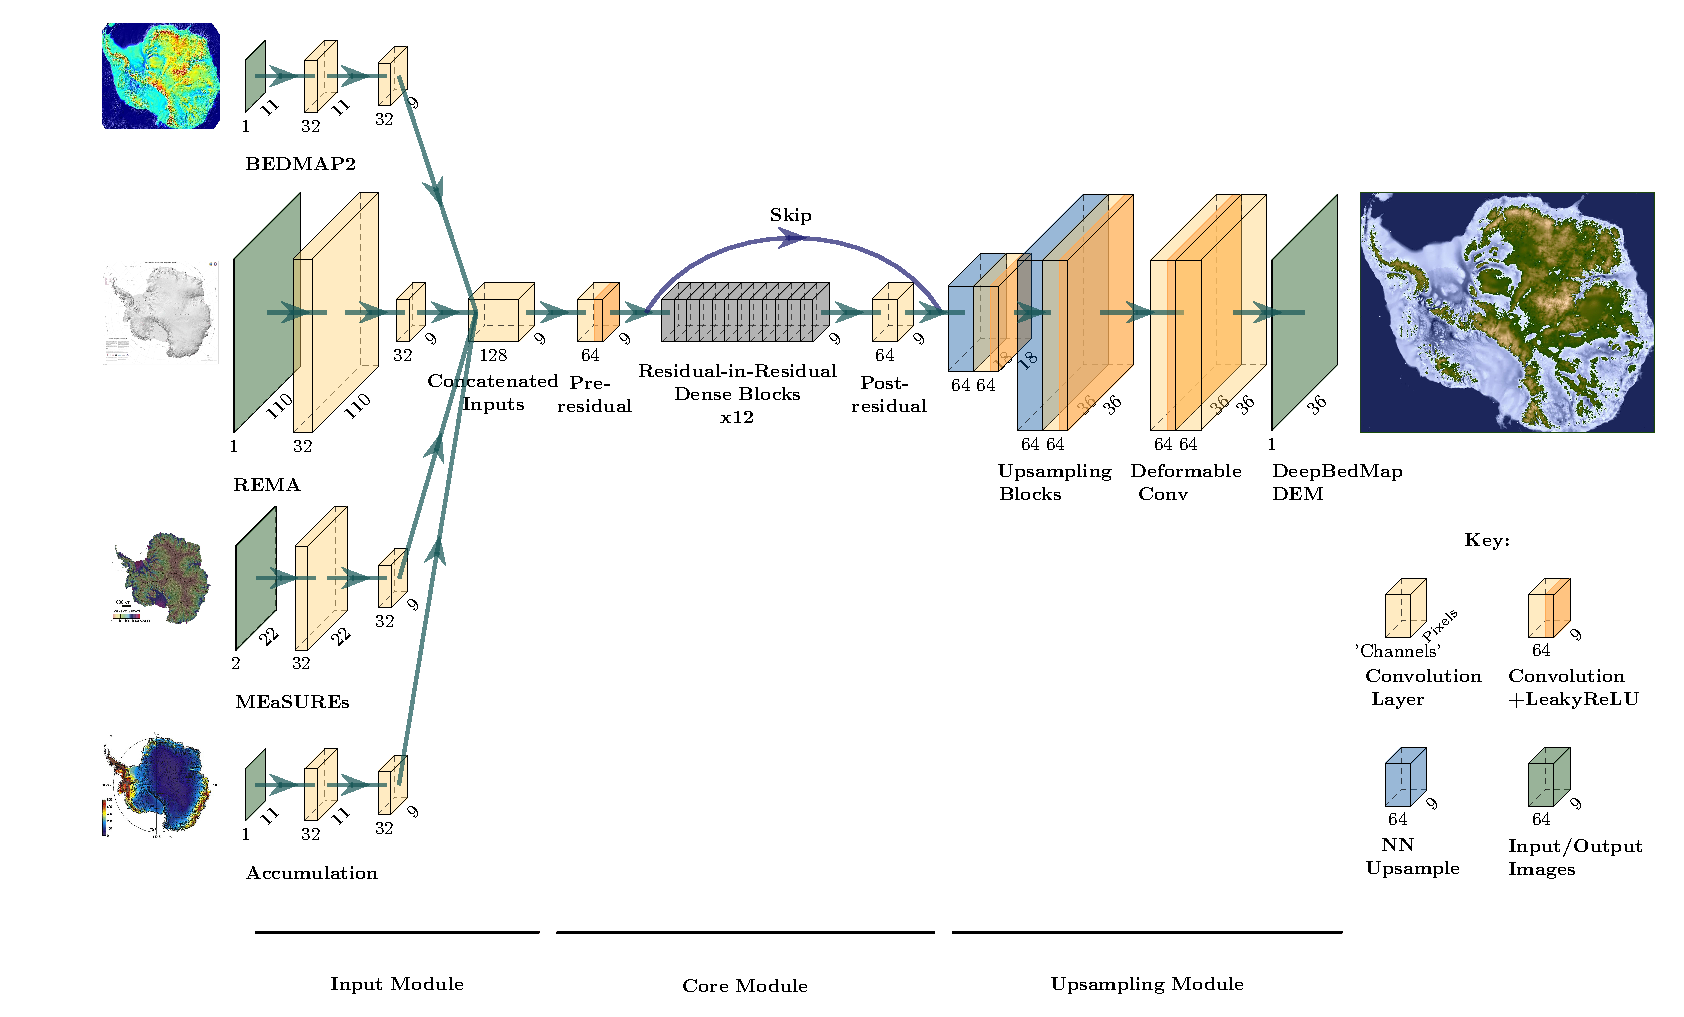
\includegraphics[width=\textwidth]{figures/fig1_deepbedmap_architecture_compressed.pdf}
  \caption{
    DeepBedMap Generator model architecture composed of three modules.
    The input module processes each of the four inputs (see Table \ref{table:datainputs}) into a consistent tensor.
    The core module processes the rich information contained within the concatenated inputs.
    The upsampling module scales the tensor up by four times and does some extra processing to produce the output DeepBedMap\_DEM.
  }
  \label{fig:1}
\end{figure*}

DeepBedMap's model architecture is adapted from the Enhanced Super Resolution Generative Adversarial Network \citep[ESRGAN,][]{WangESRGANEnhancedSuperResolution2018}.
The Generator model $G$ (see Figure \ref{fig:1}) consists of an input, core, and upsampling module.
The input module is made up of four sub-networks, each one composed of a convolutional neural network that processes the input image into a consistent 9x9 shaped tensor.
Note that the MEaSUREs Ice Velocity \citep{MouginotMEaSUREsPhaseMap2019} input has two channels, one each for the x and y velocity components.
All the processed inputs are then concatenated together channel-wise before being fed into the core module.
The core module is based on the ESRGAN architecture with 12 Residual-in-Residual Dense Blocks \citep[see][for details]{WangESRGANEnhancedSuperResolution2018}, saddled in between a pre-residual and post-residual convolutional layer.
A skip connection runs from the pre-residual layer's output to the post-residual layer's output before being fed into the upsampling module.
This skip connection \citep{HeIdentityMappingsDeep2016} helps with the neural network training process by allowing the model to also consider minimally processed information from the input module, instead of solely relying on derived information from the residual block layers when performing the upsampling.
The upsampling module is composed of two upsampling blocks, specifically a nearest neighbour upsampling followed by a convolutional layer and Leaky Rectified Linear Unit \citep[LeakyReLU,][]{MaasRectifiernonlinearitiesimprove2013} activation, that progressively scales the tensors by 2x each time.
Following this are two Deformable Convolutional layers \citep{DaiDeformableConvolutionalNetworks2017} which produces the final output super resolution DeepBedMap\_DEM.
This Generator model is trained to gradually improve its prediction by comparing the predicted output with groundtruth images in the training regions (see Figure \ref{fig:2}), using the total loss function defined in Equation \eqref{eq:A9}.

The main differences between the DeepBedMap Generator model and ESRGAN are the custom input block at the beginning, and the Deformable Convolutional layers at the end.
The custom input block is designed to handle the prior low resolution BEDMAP2 image and conditional inputs (see Table \ref{table:datainputs}).
Deformable Convolution was chosen in place of the standard Convolution so as to enhance the model's predictive capability by having it learn dense spatial transformations.

Besides the Generator model, there is a separate adversarial Discriminator model $D$ (not shown in paper).
Again, we follow ESRGAN's \citep{WangESRGANEnhancedSuperResolution2018} lead by implementing the adversarial Discriminator network in the style of the Visual Geometry Group convolutional neural network model \citep[VGG,][]{SimonyanVeryDeepConvolutional2014}.
The Discriminator model consists of 10 blocks made up of a Convolutional, Batch Normalization \citep{IoffeBatchNormalizationAccelerating2015} and LeakyReLU \citep{MaasRectifiernonlinearitiesimprove2013} layer, followed by two fully-connected layers comprised of 100 and 1 neurons respectively.
For numerical stability, we omit the final fully-connected layer's sigmoid activation function from the Discriminator model's construction, integrating it instead into the binary cross entropy loss functions at Equation \eqref{eq:A2} and Equation \eqref{eq:A3} using the log-sum-exp function.
The output of this Discriminator model is a value ranging from 0 (fake) to 1 (real) that scores the Generator model's output image.
This score is used by both the Discriminator and Generator in the training process, and helps to push the predictions towards more realistic bed elevations.
More details of the neural network training setup can be found in Appendix \ref{appendix:B}.


\section{Results}

\subsection{DeepBedMap\_DEM Topography} \label{section:deepbedmapdemtopography}

\begin{figure*}[htbp]
    \centering
    \includegraphics[width=0.75\textwidth]{figures/fig2_deepbedmap_dem_compressed.pdf}
    \caption{
      DeepBedMap\_DEM over the entire Antarctic continent.
      Plotted on an Antarctic Stereographic Projection (EPSG:3031) with elevation referenced to the WGS84 datum.
      Grounding line is plotted as thin black line.
      Purple box shows Pine Island Glacier extent used in Figure \ref{fig:3}.
      Yellow box shows Thwaites Glacier extent used in Figure \ref{fig:5}.
      Orange areas show locations of training tiles (see Table \ref{table:groundtruthdata}).
    }
    \label{fig:2}
\end{figure*}

Here we present the output Digital Elevation Model (DEM) of the super-resolution DeepBedMap neural network model, and compare it with bed topography produced by other methods.
The resulting DEM has a 250 m spatial resolution, therefore a four-times upsampled bed elevation grid product of BEDMAP2 \citep{FretwellBedmap2improvedice2013}.
In Figure \ref{fig:2}, we show that the full Antarctic-wide DeepBedMap\_DEM manages to capture general topographical features across the whole continent.
The model is only valid for grounded ice regions, but we have produced predictions extending outside of the grounding zone area (including ice shelf cavities) using the same bed elevation, surface elevation, ice velocity and snow accumulation inputs where such data is available up to the ice shelf front.
The predicted bed elevation under ice shelves is only intended to be used for visualization purposes.
Alternatively, areas of DeepBedMap\_DEM extending beyond the grounding zone can be cut out and replaced with other bathymetry grid products, using interpolation to smooth out the edges.

\begin{figure}[htbp]
  \includegraphics[width=0.75\columnwidth]{figures/fig3_qualitative_bed_comparison.png}
  \caption{
    Comparison of interpolated bed elevation grid products over Pine Island Glacier (see extent in Figure \ref{fig:2}).
    \textbf{a} DeepBedMap (ours) at 250 m resolution.
    \textbf{b} BEDMAP2 \citep{FretwellBedmap2improvedice2013}, originally 1000 m, bicubic interpolated to 250 m.
    \textbf{c} Elevation Difference between DeepBedMap and BEDMAP2.
    \textbf{d} BedMachine Antarctica \citep{MorlighemMEaSUREsBedMachineAntarctica2019}, originally 500 m, bicubic interpolated to 250 m.
  }
  \label{fig:3}
\end{figure}

We now highlight some qualitative observations of DeepBedMap\_DEM's bed topography beneath Pine Island Glacier (Figure \ref{fig:3}) and other parts of Antarctica (Figure \ref{fig:4}).
DeepBedMap\_DEM shows a terrain with realistic topographical features, having fine-scale bumps and troughs that makes it rougher than that of BEDMAP2 \citep{FretwellBedmap2improvedice2013} and BedMachine Antarctica \citep{MorlighemMEaSUREsBedMachineAntarctica2019} while still preserving the general topography of the area (Figure \ref{fig:3}).
Over steep topographical areas such as the Transantarctic Mountains (Figure \ref{fig:4}a, \ref{fig:4}h), DeepBedMap produced speckle (\textbf{S}) texture patterns.
Along fast flowing ice streams and glaciers (Figure \ref{fig:4}b, \ref{fig:4}c, \ref{fig:4}d, \ref{fig:4}e, \ref{fig:4}f, \ref{fig:4}g, \ref{fig:4}h), we can see ridges (\textbf{R}) aligned parallel to the sides of the valley, i.e. along flow.
In some cases, the ridges are also oriented perpendicular to the flow direction such at Whillans Ice Stream (Figure \ref{fig:4}b), Bindschadler Ice Stream (Figure \ref{fig:4}c) and Totten Glacier (Figure \ref{fig:4}g), resulting in intersecting ridges that creates a box-like, honeycomb structure.
Over relatively flat regions in both West and East Antarctica (e.g. Figure \ref{fig:4}g), there are some hummocky, wave-like (\textbf{W}) patterns occasionally represented in the terrain.
Terrace (\textbf{T}) features can occasionally be found winding along the side of hills such as at the Gamburtsev Subglacial Mountains (Figure \ref{fig:4}i).


\begin{figure*}[htbp]
  \includegraphics[width=\columnwidth]{figures/fig4_deepbedmap_closeups.eps}
  \caption{
    Closeup views of DeepBedMap\_DEM around Antarctica.
    Top row shows Siple Coast locations.
    Middle row shows Weddell Sea region locations.
    Bottom row shows East Antarctica locations.
    Features of interest are annotated as black text against a white background:
    Ridges \textbf{R}, Speckle patterns \textbf{S}, Terraces \textbf{T}, Wave patterns \textbf{W}.
  }
  \label{fig:4}
\end{figure*}

\subsection{Surface Roughness} \label{section:surfaceroughness}

We compare the roughness of DeepBedMap\_DEM versus BedMachine Antarctica with groundtruth grids from processed Operation IceBridge data \citep{ShiMultichannelCoherentRadar2010} using standard deviation as a simple measure of roughness \citep{RippinBasalroughnessInstitute2014}.
We calculate the surface roughness for a single 250 m pixel from the standard deviation of elevation values over a square 1250x1250 m area (i.e. 5x5 pixels) surrounding the central pixel.
Focusing on Thwaites Glacier, the spatial 2D view of the DeepBedMap\_DEM (Figure \ref{fig:5}a) shows a range of typical topographic features such as hills and canyons.
The calculated 2D roughness for both DeepBedMap\_DEM (Figure \ref{fig:5}b) and the Groundtruth (Figure \ref{fig:5}c) lie in a similar range from 0 m to 400 m whereas the roughness of BedMachine Antarctica (Figure \ref{fig:5}d) is mostly in the 0 m to 200 m range (hence the different colour scale).
Also, the roughness pattern for both DeepBedMap\_DEM and the Groundtruth has a more distributed cluster pattern made up of little pockets (especially towards the coastal region on the left, see Figure \ref{fig:5}b and \ref{fig:5}c), whereas the BedMachine Antarctica roughness pattern shows larger cluster pockets in isolated regions (see Figure \ref{fig:5}d).

\begin{figure}[htbp]
  \includegraphics[width=0.8\columnwidth]{figures/fig5_elevation_roughness_grids.eps}
  \caption{
    Spatial 2D view of grids over Thwaites Glacier, West Antarctica.
    Plotted on an Antarctic Stereographic Projection (EPSG:3031) with elevation and standard deviation values in metres referenced to the WGS84 datum.
    \textbf{a} DeepBedMap Digital Elevation Model.
    \textbf{b} 2D roughness from the DeepBedMap\_DEM grid.
    \textbf{c} 2D roughness from interpolated Operation IceBridge grid.
    \textbf{d} 2D roughness from bicubic interpolated BedMachine Antarctica grid.
    Orange points in \textbf{a} correspond to transect sampling locations used in Figure \ref{fig:6}.
    Note that color scale of \textbf{b} and \textbf{c} is two times that of \textbf{d}.
  }
  \label{fig:5}
\end{figure}

Taking a 1D transect over the 250 m resolution DeepBedMap\_DEM, BedMachine Antarctica and groundtruth grids, we illustrate the differences in bed topography and roughness from the coast towards the inland area of Thwaites Glacier with a flight trace from Operation IceBridge (see Figure \ref{fig:6}).
For better comparison, we have calculated the Operation IceBridge groundtruth bed elevation and roughness values from a resampled 250 m grid instead of using its native along-track resolution.
All three elevation profiles are shown to follow the same general trend from the relatively rough coastal region (Figure \ref{fig:6}a from -1550 to -1500 km on x-scale), along the retrograde slope (Figure \ref{fig:6}a from -1500 to -1450 km on x-scale), and into the interior region.
DeepBedMap\_DEM features a relatively noisy elevation profile with multiple fine-scale (<10 km) bumps and throughs similar to the groundtruth, while BedMachine Antarctica shows a smoother profile that is almost a moving average of the groundtruth elevation (Figure \ref{fig:6}a).
Looking at the roughness statistic (Figure \ref{fig:6}b), both the DeepBedMap\_DEM and Operation IceBridge groundtruth grids have a mean standard deviation of about 40 m whereas BedMachine Antarctica has a mean of about 10 m and rarely exceeds a standard deviation value of 20 m along the transect.

\begin{figure}[htbp]
  \includegraphics[width=0.9\columnwidth]{figures/fig6_elevation_roughness_transect.eps}
  \caption{
    Comparing bed elevation \textbf{a} and surface roughness \textbf{b} (standard deviation of elevation values) of each interpolated grid product (250 m resolution) over a transect (see Figure \ref{fig:5} for location of transect line).
    Purple values are from the super resolution DeepBedMap\_DEM;
    Orange values are from tension spline interpolated Operation IceBridge groundtruth points;
    Green values are from bicubic interpolated BedMachine Antarctica.
  }
  \label{fig:6}
\end{figure}


\section{Discussion}

\subsection{Interpretation}

In Section \ref{section:deepbedmapdemtopography}, we show that the DeepBedMap model has produced a high resolution (250 m) result (see Figure \ref{fig:3}) that can capture a detailed and realistic picture of the underlying bed topography.
The fine scale bumps and troughs are the result of the DeepBedMap Generator model learning to produce features that are similar to those found in the high resolution groundtruth datasets it was trained on.
However, there are also artifacts produced by the model.
For example, the winding terrace (\textbf{T}, Figure \ref{fig:4}) features are hard to explain, and though they resemble eskers \citep{DrewsActivelyevolvingsubglacial2017}, their placement along the sides of hills does not support this view.
Similarly, we are not sure why speckle (\textbf{S}, Figure \ref{fig:4}) texture patterns are found over steep mountains, but the lack of high resolution training datasets likely leads the model to perform worse over these high gradient areas.

Another issue is that DeepBedMap will often pick up details from the high resolution ice surface elevation model \citep{HowatReferenceElevationModel2019} input dataset, which may not be representative of the true bed topography.
For example, the ridges (\textbf{R}, Figure \ref{fig:4}) found along fast flowing ice streams and glaciers are likely to be the imprints of crevasses or flowstripes \citep{GlasserLongitudinalsurfacestructures2012} observable from the surface.
An alternative explanation is that the ridges, especially the honeycomb-shaped ones, are rhombohedral moraine deposits formed by soft sediment squeezed up into basal crevasses that are sometimes found at stagnant surging glaciers \citep{Dowdeswellvarietydistributionsubmarine2016,DowdeswellRhombohedralcrevassefillridges2016,SolheimSeafloormorphologyoutside1985}.
We favour the first intepretation as the positions of these bed features coincide with the surface features, and also because these ridges are more likely to be eroded away in these fast flowing ice stream areas.

The hummocky wave-like (\textbf{W}) patterns we observe over the relatively flat and slower flowing areas are likely to result from surface megadune structures \citep{ScambosSnowMegadune2014}.
Alternatively, they may be ribbed or rogen morraine features that are formed in an orientation transverse to the ice flow direction  \citep{HattestrandRibbedmorainesSweden1997,HattestrandRibbedmoraineformation1999}.
While any one of these two explanations may be valid in different regions of Antarctica, we lean towards the conservative interpretation that these features are the result of the DeepBedMap model overfitting to the ice surface elevation data.

In Section \ref{section:surfaceroughness}, we quantify that a well trained DeepBedMap neural network model can produce high roughness values more comparable to the groundtruth than BedMachine Antarctica.
While the mass conservation technique used by BedMachine Antarctica \citep{MorlighemDeepglacialtroughs2019} improves upon ordinary interpolation techniques such as bicubic interpolation and kriging, their results are still inherently smooth by nature.
The groundtruth grids show that rough areas do exist on a fine scale, and so the high resolution models we produce should reflect that.

DeepBedMap\_DEM manages to capture much of the rough topography found in the Operation IceBridge groundtruth data, especially near the coast (see Figure \ref{fig:6}a, from -1550 to -1500 km on x-scale) where the terrain tends to be rougher.
Along the retrograde slope (see Figure \ref{fig:6}a, from -1500 to -1450 km on x-scale), several of the fine-scale (<10 km) bumps and troughs in DeepBedMap\_DEM can be seen to correlate well in position with the groundtruth.
In contrast, the cubic interpolated BedMachine Antarctica product lacks such fine-scale (<10 km) bumps and troughs, appearing as a relatively smooth terrain over much of the transect.
Previous studies that estimated basal shear stress over Thwaites Glacier have found a band of strong bed extending about 80-100 km from the grounding line, with pockets of weak bed interspersed between bands of strong bed further upstream \citep{JoughinBasalconditionsPine2009,SergienkoRegularPatternsFrictional2013}, a pattern that is broadly consistent with the DeepBedMap\_DEM roughness results (see Figure \ref{fig:5}b).
In general, DeepBedMap\_DEM produces a topography that is much more rougher, with standard deviation values more in line with those observed in the groundtruth (see Figure \ref{fig:6}b).
The roughness values for BedMachine Antarctica are consistently lower throughout the transect, a consequence of the mass conservation technique using regularization parameters that yields smooth results.
Recent studies have stressed the importance of form drag (basal drag due to bed topography) over skin drag (or basal friction) on the basal traction of Pine Island Glacier \citep{BinghamDiverselandscapesPine2017,Kyrke-SmithRelevanceDetailBasal2018}, and the DeepBedMap super-resolution work here shows strong potential in meeting that demand as a realistic high resolution bed topography dataset for ice sheet modelling studies.

\subsection{Limitations}

The DeepBedMap model is trained only on a small fraction of the area of Antarctica, simply because the convolutional neural network cannot be trained on sparse survey point measurements.
The topography generated by the model is quite sensitive to the accuracy of its data inputs (see Table \ref{table:groundtruthdata} and \ref{table:datainputs}), and though this is a problem faced by many other inverse methods, neural network models like ours can be particularly biased towards the training dataset.

An inherent assumption in this methodology is that the training data sets have sampled the variable bed lithology of Antarctica \citep{CoxGeoMAPdatasetAntarctic2018} sufficiently.
This is unlikely to be true, introducing uncertainty in the result as different lithologies may cause the same macro-scale bed landscapes to result in a range of surface features.
In particular, the experimental model's topography is likely skewed towards the distribution of the training regions that tend to reside in coastal regions, especially over ice streams in West Antarctica (see Figure \ref{fig:2}).
Besides collecting more radio-echo sounding datasets to sample these regions more densely, swath reprocessing of old datasets that have that capability \citep{HolschuhSwathtopographyfuture2019} may be another useful addition to the training set.

\subsection{Future directions}

While care has been taking to source the best possible datasets (see Table \ref{table:groundtruthdata} and \ref{table:datainputs}), we note that there is still room to improve the DeepBedMap\_DEM's results.
Some of the conditional datasets we use such as REMA \citep{HowatReferenceElevationModel2019} and MEaSUREs Ice Velocity \citep{MouginotMEaSUREsPhaseMap2019} contain data gaps which introduce artifacts in the DeepBedMap\_DEM, and those holes need to be patched up for proper continent-wide prediction.
As the DeepBedMap model relies on data from multiple sources which are collected over different epochs, it has no proper sense of time.
Ice elevation change captured using satellite altimeters (e.g. from ICESat-2 \citep{MarkusIceCloudland2017}) could be added as an additional input to better account for temporal factors.
It is possible to apply the super resolution DeepBedMap technique on bed elevation inputs newer than BEDMAP2 \citep{FretwellBedmap2improvedice2013}, such as the 1000 m resolution DEM over the Weddell Sea \citep{Jeofry1KmBedTopography2017} or the 500 m resolution Bedmachine Antarctica dataset \citep{MorlighemMEaSUREsBedMachineAntarctica2019}.

Our DeepBedMap model is modular by design, and the different modules (see Figure \ref{fig:1}) can be improved on and adapted for future use cases.
The architecture of the input module can be modified to handle new datasets such as the ones suggested above, or redesigned to extract a greater amount of information for better performance.
Similarly, the core and upsampling modules which are based on ESRGAN \citep{WangESRGANEnhancedSuperResolution2018} can be replaced with newer, better architectures as the need arises.
The redesigned neural network model can be retrained from scratch or fine-tuned using the trained weights from DeepBedMap to further improve the predictive performance.
Taken together, these advances will lead to an even more accurate and higher resolution bed elevation model.


\conclusions  %% \conclusions[modified heading if necessary]

The DeepBedMap convolutional neural network method presents a data-driven approach to better resolve the bed topography of Antarctica using existing data.
It is an improvement beyond simple interpolation techniques, generating realistic high spatial resolution (250 m) topography that preserves detail in bed roughness and is adaptable for catchment to continent-scale studies on ice sheets.
Unlike other inverse methods that rely on some explicit parameterization of ice-flow physics, the model uses deep learning to find suitable neural network parameters via an iterative error minimization approach.
This makes the resulting model particularly sensitive to the training data set, emphasizing the value of densely spaced bed elevation datasets and the need for such sampling over a more diverse range of Antarctic substrate types.
The use of Graphical Processing Units (GPUs) for training and inference allows the neural network method to scale easily, and the addition of more training datasets will allow it to perform better.

The work here is not intended to discourage the usage of other inverse modelling techniques, but to introduce an independent methodology, with an outlook towards combining the strengths of the two.
Once properly trained, the DeepBedMap model runs quickly and produces realistic rough topography, which when merged with more physically based mass conservation inverse approaches \citep[e.g.][]{MorlighemDeepglacialtroughs2019} will likely result in more efficient ways of generating accurate bed elevation maps of Antarctica.
One side product resulting from this work is a test-driven development framework that can be used to measure and compare the performance of upcoming bed terrain models.
The radioglaciology community has already begun to compile a new comprehensive bed elevation/ice thickness dataset for Antarctica, and there has been discussions to combine various terrain interpolation techniques in an ensemble to collaboratively create the new BEDMAP3.




%% The following commands are for the statements about the availability of data sets and/or software code corresponding to the manuscript.
%% It is strongly recommended to make use of these sections in case data sets and/or software code have been part of your research the article is based on.

\codeavailability{
  Python code for data preparation, neural network model training and visualization of model outputs are freely available at https://github.com/weiji14/deepbedmap.
  Neural network model training experiment runs are also recorded at https://www.comet.ml/weiji14/deepbedmap.
} %% use this section when having only software code available


\dataavailability{
  DeepBedMap\_DEM available through the Open Science Framework platform at https://doi.org/10.17605/OSF.IO/96APW.
  Pine Island Glacier dataset \citep{BinghamDiverselandscapesPine2017} available on request from Robert Bingham.
  Carlson Inlet dataset \citep{KingIcestreamnot2011} available on request from Edward King.
  Bed elevation datasets from Wilkes Subglacial Basin \citep{FerraccioliAirborneradarbed2018} and Rutford Ice Stream \citep{KingSubglaciallandformsRutford2016} available from British Antarctic Survey's Polar Data Centre (https://ramadda.data.bas.ac.uk).
  Other Antarctic bed elevation datasets available from Center for Remote Sensing of Ice Sheets (https://data.cresis.ku.edu/data/rds) or from National Snow and Ice Data Center (https://nsidc.org/data/IRMCR2/versions/1).
  BEDMAP2 \citep{FretwellBedmap2improvedice2013} and REMA \citep{HowatReferenceElevationModel2018} available from Polar Geospatial Center (http://data.pgc.umn.edu).
  MEaSUREs ice velocity data \citep{MouginotMEaSUREsPhaseMap2019} available from NSIDC (https://nsidc.org/data/nsidc-0754/versions/1).
  Antarctic Snow Accummulation data \citep{ArthernAntarcticsnowaccumulation2006} available from British Antarctic Survey (https://secure.antarctica.ac.uk/data/bedmap2/resources/Arthern\_accumulation).
} %% use this section when having only data sets available


% \codedataavailability{TEXT} %% use this section when having data sets and software code available


% \sampleavailability{TEXT} %% use this section when having geoscientific samples available


% \videosupplement{TEXT} %% use this section when having video supplements available


\appendix

\section{Details of loss function components} \label{appendix:A}

The loss function, or cost function, is a mathematical function that maps a set of input variables to an output loss value.
The loss value can be thought of as a weighted sum of several error metrics between the neural network's prediction and the expected output or groundtruth.
It is this loss value which we want to minimize so as to train the neural network model to perform better, and we do this by iteratively optimizing the parameters in the loss function.
Following this are the details of the various loss functions that make up the total loss function of the DeepBedMap Generative Adversarial Network model.

\subsection{Content Loss}

To bring the pixel values of the generated images closer to that of the groundtruth, we first define the Content Loss function $L_1$.
Following ESRGAN \citep{WangESRGANEnhancedSuperResolution2018}, we have:

\begin{equation}\label{eq:A1}
  L_1 = \dfrac{1}{n} \sum\limits_{i=1}^n ||\hat{y}_i - y_i||_{1}
\end{equation}

where we take the mean absolute error between the Generator Network's predicted value $\hat{y}_i$ and the groundtruth value $y_i$, respectively over every pixel $i$.

\subsection{Adversarial Loss}

Next, we define an Adversarial Loss to encourage the production of high resolution images $\hat{y}$ closer to the manifold of natural looking digital elevation model images.
To do so, we introduce the standard discriminator in the form of $D(y) = \sigma(C(y))$ where $\sigma$ is the sigmoid activation function and $C(y)$ is the raw, non-transformed output from a discriminator neural network acting on high resolution image $y$.
The ESRGAN model \citep{WangESRGANEnhancedSuperResolution2018} however, employs an improved Relativistic-average Discriminator \citep{Jolicoeur-Martineaurelativisticdiscriminatorkey2018} denoted by $D_{Ra}$.
It is defined as $D_{Ra}(y,\hat{y}) = \sigma(C(y) - \mathbb{E}_{\hat{y}}[C(\hat{y})])$, where $\mathbb{E}_{\hat{y}}[\cdot]$ is the arithmetic mean operation carried out over every generated image $\hat{y}$ in a mini-batch.
We use a binary cross entropy loss as the discriminator's loss function defined as follows:

\begin{equation}\label{eq:A2}
  L_D^{Ra} = - \mathbb{E}_y[\ln(D(y,\hat{y}))] - \mathbb{E}_{\hat{y}}[\ln(1 - D(\hat{y},y))]
\end{equation}

The generator network's adversarial loss is in a symmetrical form:

\begin{equation}\label{eq:A3}
  L_G^{Ra} = - \mathbb{E}_y[\ln(1 - D(y,\hat{y}))] - \mathbb{E}_{\hat{y}}[\ln(D(\hat{y},y))]
\end{equation}

\subsection{Topographic Loss}

We further define a Topographic Loss so that the elevation values in the super resolved image make topographic sense with respect to the original low resolution image.
Specifically, we want the mean value of each 4x4 grid on the predicted super resolution (DeepBedMap) image to closely match its spatially corresponding 1x1 pixel on the low resolution (BEDMAP2) image.

First, we apply a 4x4 Mean Pooling operation on the Generator Network's predicted super resolution image:

\begin{equation}\label{eq:A4}
 \bar{\hat{y}}_j = \dfrac{1}{n} \sum\limits_{i=1}^n \hat{y}_i
\end{equation}

where $\bar{\hat{y}}_j$ is the mean of all predicted values $\hat{y}_i$ across the 16 super-resolved pixels $i$ within a 4x4 grid corresponding to the spatial location of one low resolution pixel at position $j$.
Following this, we can compute the Topographic Loss as follows:

\begin{equation}\label{eq:A5}
  L_T = \dfrac{1}{m} \sum\limits_{i=1}^m ||\bar{\hat{y}}_j - x_j||_{1}
\end{equation}

where we take the mean absolute error between the mean of the 4x4 super-resolved pixels calculated in Equation \eqref{eq:A4} $\bar{\hat{y}}_j$ and that of the spatially corresponding low resolution pixel $x_j$, respectively over every low resolution pixel $j$.

\subsection{Structural Loss}

Lastly, we define a Structural Loss that takes into account luminance, contrast and structural information between the predicted and groundtruth images.
This is based on the Structural Similarity Index \citep[SSIM,][]{WangImageQualityAssessment2004} and is calculated over a single window patch as so:

\begin{equation}\label{eq:A6}
  SSIM(\hat{y}, y) = \dfrac{(2\mu_{\hat{y}}\mu_y + c_1)(2\sigma_{{\hat{y}}y} + c_2)}{(\mu_{\hat{y}}^2 + \mu_y^2 + c_1)(\sigma_{\hat{y}}^2 + \sigma_y^2 + c_2)}
\end{equation}

where $\mu_{\hat{y}}$ and $\mu_y$ are the arithmetic mean of predicted image ${\hat{y}}$ and groundtruth image $y$ respectively over a single window that we set to 9x9 pixels, $\sigma_{{\hat{y}}y}$ is the covariance of ${\hat{y}}$ and $y$, $\sigma_{\hat{y}}^2$ and $\sigma_y^2$ are the variance of ${\hat{y}}$ and $y$ respectively, and $c_1$ and $c_2$ are two variables set to $0.01^2$ and $0.03^2$ to stabilize division with a weak denominator.
Thus, we can formulate the Structural Loss as follows:

\begin{equation}\label{eq:A7}
  L_S = 1 - \dfrac{1}{p} \sum\limits_{i=1}^p SSIM(\hat{y}, y)_p
\end{equation}

where we do $1$ minus the mean of all structural similarity values $SSIM(\hat{y}, y)$ calculated over every patch $p$ obtained via a sliding window over the predicted image ${\hat{y}}$ and groundtruth image $y$.

\subsection{Total Loss Function}

Finally, we compile the loss functions for the discriminator and generator networks as follows:

\begin{align}
  & L_D = L_D^{Ra} \label{eq:A8}\\
  & L_G = \eta L_1 + \lambda L_G^{Ra} + \theta L_T + \zeta L_S \label{eq:A9}
\end{align}

where $\eta$, $\lambda$, $\theta$, and $\zeta$ are the scaled weights for the content $L_1$, adversarial $L_D$, topographic $L_T$ and structural losses $L_S$ respectively (see Table \ref{table:B1} for values used).
The loss functions $L_D$ and $L_G$ are minimized in an alternate 1:1 manner so as to solve the entire Generative Adversarial Network's objective function defined in Equation \eqref{eq:4}.


\section{Neural Network Training Details} \label{appendix:B}

The neural networks were developed using Chainer v7.0.0b2 \citep{TokuiChainerDeepLearning2019}, and trained using full precision (floating point 32) arithmetic.
Experiments were carried out on 4 Graphical Processing Units (GPUs), specifically 2 Tesla P100 GPUs and 2 Tesla V100 GPUs.
On the Tesla V100 GPU setup, one training run with about 150 epochs takes about 30 minutes.
This is using a batch size of 128 on a total of 3826 training image tiles, with 202 tiles reserved for validation, i.e. a 95/5 training/validation split.
We next describe the method used to evaluate each DeepBedMap candidate model, as well as the high-level way in which we semi-automatically arrived at a good model via semi-automatic hyperparameter tuning.

\begin{table*}[htbp]
  \caption{Optimized Hyperparameter Settings.}
  \label{table:B1}
  \begin{tabular}{lrr}
  \tophline
  Hyperparameter & Setting & Tuning Range \\
  \middlehline
  Learning rate (for both Generator and Discriminator) & 1.7e-4 & 2e-4 to 1e-4 \\
  Number of Residual-in-Residual Blocks & 12 & 8 to 14 \\
  Mini-batch size & 128 & 64 or 128 \\
  Number of epochs & 140 & 90 to 150 \\
  Residual scaling & 0.2 & 0.1 to 0.5 \\
  Content Loss Weighting $\eta$ & 1e-2 & Fixed \\
  Adversarial Loss Weighting $\lambda$ & 2e-2 & Fixed \\
  Topographic Loss Weighting $\theta$ & 2e-3 & Fixed \\
  Structural Loss Weighting $\zeta$ & 5.25 & Fixed \\
  He Normal Initialization Scaling & 0.1 & Fixed \\
  Adam optimizer epsilon & 0.1 & Fixed \\
  Adam optimizer beta1 & 0.9 & Fixed \\
  Adam optimizer beta2 & 0.99 & Fixed \\
  \bottomhline
  \end{tabular}
  \belowtable{} % Table Footnotes
\end{table*}

To check for overfitting, we evaluate the Generative Adversarial Network model on the validation dataset after each epoch using two performance metrics - a peak signal-to-noise ratio (PSNR) metric for the Generator, and an accuracy metric for the Discriminator.
Training stops when these validation performance metrics show little improvement, roughly at 120 epochs.

Next, we conduct a full evaluation on an independent test dataset, comparing the model's predicted grid output against actual groundtruth xyz points.
Using the `grdtrack' function in Generic Mapping Tools v6.0 \citep{WesselGenericMappingTools2019}, we obtain the grid elevation at each groundtruth point and use it to calculate the elevation error on a point-to-point basis.
All of these elevation errors are then used to compute a Root Mean Squared Error (RMSE) statistic over this independent test site.
This RMSE value is used to judge the model's performance in relation to baseline bicubic interpolation, and also the metric minimized by a hyperparameter optimization algorithm which we will describe next.

Neural networks contain a lot of hyperparameter settings that need to be decided upon, and Generative Adversarial Networks are particularly sensitive to different hyperparameter settings.
To stabilize model training and obtain better performance, we tune the hyperparameters (see Table \ref{table:B1}) using a Bayesian approach.
Specifically, we employ the Tree-structured Parzen Estimator \citep{BergstraAlgorithmsHyperparameterOptimization2011} from the Optuna v0.14.0 \citep{AkibaOptunaNextgenerationHyperparameter2019} library with default settings as per the Hyperopt library \citep{BergstraHyperoptPythonlibrary2015}.
Given that we have 4 GPUs, we choose to parallelize the hyperparameter tuning experiments asynchronously between all four devices.
The estimator first conducts 20 random experimental trials to scan the hyperparameter space, gradually narrowing down to a few candidate hyperparameters in subsequent experiments.
We set each GPU to run a target of 30 experimental trials (i.e. a total of 120), though unpromising trials that have exploding/vanishing gradients are pruned prematurely to save on time and computational resources.
The top models from these experiments undergo further visual evaluation, and we continue to conduct further experiments until a suitable candidate model is found.

\noappendix       %% use this to mark the end of the appendix section. Otherwise the figures might be numbered incorrectly (e.g. 10 instead of 1).

%% Regarding figures and tables in appendices, the following two options are possible depending on your general handling of figures and tables in the manuscript environment:

%% Option 1: If you sorted all figures and tables into the sections of the text, please also sort the appendix figures and appendix tables into the respective appendix sections.
%% They will be correctly named automatically.

%% Option 2: If you put all figures after the reference list, please insert appendix tables and figures after the normal tables and figures.
%% To rename them correctly to A1, A2, etc., please add the following commands in front of them:

\appendixfigures  %% needs to be added in front of appendix figures

\appendixtables   %% needs to be added in front of appendix tables

%% Please add \clearpage between each table and/or figure. Further guidelines on figures and tables can be found below.



\authorcontribution{
  W. J. L. - conceptualisation, data curation, formal analysis, methodology, software, visualization, writing – original draft, writing – review \& editing.
  H. J. H. - conceptualisation, funding acquisition, supervision, writing – review \& editing.
} %% this section is mandatory

\competinginterests{The authors declare that they have no conflict of interest.} %% this section is mandatory even if you declare that no competing interests are present

% \disclaimer{TEXT} %% optional section

\begin{acknowledgements}
  We are grateful to Robert Bingham and Edward King for the Pine Island Glacier and Carlson Inlet data, and to all the other researchers in the British Antarctic Survey and Operation IceBridge team for providing free access to the high resolution bed elevation datasets around Antarctica.
  A special thanks to Ruzica Dadic for her help in reviewing draft versions of this paper.
  This research was funded by the Royal Society of New Zealand's Rutherford Discovery Fellowship (Contract: RDF‐VUW1602), with additional support from the Erasmus+ programme and International Glaciological Society early career travel award for presenting earlier versions of this work at the 2019 EGU General Assembly and IGS Symposium on Five Decades of Radioglaciology.
\end{acknowledgements}




%% REFERENCES

%% The reference list is compiled as follows:

%% \begin{thebibliography}{}

%% \bibitem[AUTHOR(YEAR)]{LABEL1}
%% REFERENCE 1

%% \bibitem[AUTHOR(YEAR)]{LABEL2}
%% REFERENCE 2

%% \end{thebibliography}

%% Since the Copernicus LaTeX package includes the BibTeX style file copernicus.bst,
%% authors experienced with BibTeX only have to include the following two lines:
%%
\bibliographystyle{copernicus}
\bibliography{example.bib}
%%
%% URLs and DOIs can be entered in your BibTeX file as:
%%
%% URL = {http://www.xyz.org/~jones/idx_g.htm}
%% DOI = {10.5194/xyz}


%% LITERATURE CITATIONS
%%
%% command                        & example result
%% \citet{jones90}|               & Jones et al. (1990)
%% \citep{jones90}|               & (Jones et al., 1990)
%% \citep{jones90,jones93}|       & (Jones et al., 1990, 1993)
%% \citep[p.~32]{jones90}|        & (Jones et al., 1990, p.~32)
%% \citep[e.g.,][]{jones90}|      & (e.g., Jones et al., 1990)
%% \citep[e.g.,][p.~32]{jones90}| & (e.g., Jones et al., 1990, p.~32)
%% \citeauthor{jones90}|          & Jones et al.
%% \citeyear{jones90}|            & 1990



%% FIGURES

%% When figures and tables are placed at the end of the MS (article in one-column style), please add \clearpage
%% between bibliography and first table and/or figure as well as between each table and/or figure.

% The figure files should be labelled correctly with Arabic numerals (e.g. fig01.jpg, fig02.png).


%% ONE-COLUMN FIGURES

%%f
%\begin{figure}[t]
%\includegraphics[width=8.3cm]{FILE NAME}
%\caption{TEXT}
%\end{figure}
%
%%% TWO-COLUMN FIGURES
%
%%f
%\begin{figure*}[t]
%\includegraphics[width=12cm]{FILE NAME}
%\caption{TEXT}
%\end{figure*}
%
%
%%% TABLES
%%%
%%% The different columns must be seperated with a & command and should
%%% end with \\ to identify the column brake.
%
%%% ONE-COLUMN TABLE
%
%%t
%\begin{table}[t]
%\caption{TEXT}
%\begin{tabular}{column = lcr}
%\tophline
%
%\middlehline
%
%\bottomhline
%\end{tabular}
%\belowtable{} % Table Footnotes
%\end{table}
%
%%% TWO-COLUMN TABLE
%
%%t
%\begin{table*}[t]
%\caption{TEXT}
%\begin{tabular}{column = lcr}
%\tophline
%
%\middlehline
%
%\bottomhline
%\end{tabular}
%\belowtable{} % Table Footnotes
%\end{table*}
%
%%% LANDSCAPE TABLE
%
%%t
%\begin{sidewaystable*}[t]
%\caption{TEXT}
%\begin{tabular}{column = lcr}
%\tophline
%
%\middlehline
%
%\bottomhline
%\end{tabular}
%\belowtable{} % Table Footnotes
%\end{sidewaystable*}
%
%
%%% MATHEMATICAL EXPRESSIONS
%
%%% All papers typeset by Copernicus Publications follow the math typesetting regulations
%%% given by the IUPAC Green Book (IUPAC: Quantities, Units and Symbols in Physical Chemistry,
%%% 2nd Edn., Blackwell Science, available at: http://old.iupac.org/publications/books/gbook/green_book_2ed.pdf, 1993).
%%%
%%% Physical quantities/variables are typeset in italic font (t for time, T for Temperature)
%%% Indices which are not defined are typeset in italic font (x, y, z, a, b, c)
%%% Items/objects which are defined are typeset in roman font (Car A, Car B)
%%% Descriptions/specifications which are defined by itself are typeset in roman font (abs, rel, ref, tot, net, ice)
%%% Abbreviations from 2 letters are typeset in roman font (RH, LAI)
%%% Vectors are identified in bold italic font using \vec{x}
%%% Matrices are identified in bold roman font
%%% Multiplication signs are typeset using the LaTeX commands \times (for vector products, grids, and exponential notations) or \cdot
%%% The character * should not be applied as mutliplication sign
%
%
%%% EQUATIONS
%
%%% Single-row equation
%
%\begin{equation}
%
%\end{equation}
%
%%% Multiline equation
%
%\begin{align}
%& 3 + 5 = 8\\
%& 3 + 5 = 8\\
%& 3 + 5 = 8
%\end{align}
%
%
%%% MATRICES
%
%\begin{matrix}
%x & y & z\\
%x & y & z\\
%x & y & z\\
%\end{matrix}
%
%
%%% ALGORITHM
%
%\begin{algorithm}
%\caption{...}
%\label{a1}
%\begin{algorithmic}
%...
%\end{algorithmic}
%\end{algorithm}
%
%
%%% CHEMICAL FORMULAS AND REACTIONS
%
%%% For formulas embedded in the text, please use \chem{}
%
%%% The reaction environment creates labels including the letter R, i.e. (R1), (R2), etc.
%
%\begin{reaction}
%%% \rightarrow should be used for normal (one-way) chemical reactions
%%% \rightleftharpoons should be used for equilibria
%%% \leftrightarrow should be used for resonance structures
%\end{reaction}
%
%
%%% PHYSICAL UNITS
%%%
%%% Please use \unit{} and apply the exponential notation


\end{document}
